\documentclass{article}
\usepackage{amsmath}
\usepackage{amssymb}
\usepackage{microtype}
\usepackage{graphicx}
\usepackage{subfigure}
\usepackage{booktabs} % for professional tables


\usepackage{hyperref}
\usepackage{array}

% Attempt to make hyperref and algorithmic work together better:
\newcommand{\theHalgorithm}{\arabic{algorithm}}

\usepackage[accepted]{icml2021}

% The \icmltitle you define below is probably too long as a header.
% Therefore, a short form for the running title is supplied here:
\icmltitlerunning{Image Animation with Keypoint Mask}

\begin{document}

\twocolumn[
\icmltitle{Image Animation with Keypoint Mask}

\icmlsetsymbol{equal}{*}

\begin{icmlauthorlist}
\icmlauthor{Or Toledano}{tlv}
\icmlauthor{Yanir Marmor}{tlv}
\icmlauthor{Dov Gertz}{tlv}

\end{icmlauthorlist}

\icmlaffiliation{tlv}{Tel Aviv University}

\icmlcorrespondingauthor{Or Toledano}{ortoledano@protonmail.com}
\icmlcorrespondingauthor{Yanir Marmor}{yanirmr@gmail.com}
\icmlcorrespondingauthor{Dov Gertz}{dovgertz1@gmail.com}


\icmlkeywords{Machine Learning, ICML}

\vskip 0.3in
]
\printAffiliationsAndNotice{}

\begin{abstract}
Motion transfer is the task of synthesizing future video frames of a single
source image according to the motion from a given driving video.
This task is challenging due to the complexity of motion representation
and the unknown relations between the driving video and the source image.
Despite this difficulty, this problem attracted great interests from
researches at the recent years, with gradual improvements. The
problem can be thought as decoupling of motion and appearance, which is
often solved by extracting the motion from keypoint movement.
We chose to use the generic, unsupervised setting, so we can apply
animation to any arbitrary object, without any domain specific model for the
structure of the input.
In this work, we extract the structure from a keypoint heatmap, without an
explicit motion representation. Then, the structures from the image and the video
are extracted to warp the image according to the video, by a deep
generator.
\end{abstract}

\section{Introduction}

TODO: add here table with to rows - one of original video and the other with generated one - on the same movement. this is our click-bite!

Take a look at Figure 1 for two video sequences. The input is a YouTube clip of a Thai-Chi artist(?) (the source subject) performing a series of motions in the top row. Our algorithm's output is shown in the bottom row. It refers to frames that appear to show a different person (the target subject) executing the same motions. The twist is that the target individual has never performed the same exact sequence of motions as the source. In reality, he was photographed another movement with no clear reference to the source's actions.
And, as the figure shows, the source and the target are of different races, have different builds, and dress differently.

In this study, we propose a simple, however surprisingly efficient approach to video retargeting – the transfer of the movement automatically from driving video sequence trough an source image for a new artificial video. Two inputs – image of the target person whose appearance we want to summarize and the other one of the source theme, the motion of which we want to impose on our target person – allow us to transfer movement between them by learning a compact motion representation.
With our framework, we create a variety of videos that never even happen.

A lot of researches observe that the keypoint-based pose maintains motion
signatures over time, while abstracting all possible subject identities as
much as possible. We therefore use the keypoint-based pattern in more "soft" way. We balanced the key points in such a way that delicate movements could be restored with great precision.

The main challenges we need to deal with, as they defined in that survey are: paired training, identity leakage, occlusions and temporal coherence,

TODO: does the next paragraph required?

Our paper focuses on the motion transfer problem: given a source image $S$
and a driving video $D$, the goal is to synthesize a video with the identity
of $S$, and the motion from $D$.
Some notable works \cite{siarohin2020order}, \cite{wiles2018x2face},
\cite{siarohin2019animating}.

TODO: does the next line required?
Our method does not rely on GANs - see Section~\ref{method}.

TODO: I think we need to write the next pragraph with more juicy details. I wrote this too much laocnic.

Our contribution it twofold: first, show that reducing the motion prior can
work and yield better accuracy results, and second compact representation with better performance.

\medskip

\textbf{Related Work:}
Motion transfer has gained a lot of coverage over the last twenty years. Early approaches based on manipulating existing video footage to generate new content. They searched for frames in which the body position corresponded to the desired motion and use them to generate a new content\cite{bregler1997video}. Our approach is equally designed for videos, but rather than manipulating existing images, we learn to synthesize new movements that never was done.

A number of techniques are based on calibrated multi camera systems to scan a target player and use an adapted 3D model of the target to control their motion in a new frame\cite{cheung2004markerless}. Our solution instead examines the transition of movement between 2D video subjects and prevents data calibration or 3D space boost.

Deep learning for reanimation has been used in many implementations in recent works and relies on more accurate input representations. Due to the synthetic rendering, an interior model and a gaze map as an input. They manage to transfer head position and facial expressions among human subjects and to produce detailed portrait videos of their facial gestures\cite{kim2018deep}. Our problem is similar to that, except that our is full body movement  redirected and the inputs to our model are 2D video and an image. No external data replication is used.

Latest approaches concentrate on the disentangling of appearance and activity and synthesizing of new motion videos \cite{tulyakov2018mocogan}. Similarly, we apply
our representation of motion to different target subjects to
generate new motions. However, in contrast to these  general methods we specialize on synthesizing detailed martial art videos.

TODO: how do you think we need to finish this section?

Our work doesn't rely directly on a strong motion prior,
but uses a structure mask which was extracted from a keypoint detector
of a motion based model, such as \cite{siarohin2020order}. The concept of using drawn keypoints as
a geometry representation (structural mask) was already used in the context
of image-to-image translation, in works such as TransGaGa \cite{wu2019transgaga}.
The concept of using a structural mask in the context of image animation is
demonstrated in \cite{shalev2020image}. However, the current work differs
by basing the mask off a motion related module, which saves us the hassle
of perturbing the input hoping to achieve an identity-less mask which might
not even be optimal. That way, we
can base more of the motion representation on the deep network, reduce our
prior, and leave some space for our network to achieve better results.


\subsection{Keypoints}
In contrast to pixel-based approaches that were prevalent until a few years
ago, recently, keypoint-based approaches have been perceived as having the
potential to achieve high performance in the field of video reanimation. Some recent works that use this method are:
\cite{kim2019unsupervised}, \cite{balakrishnan2018synthesizing}
\cite{ma2017pose}  \cite{reed2017parallel} \cite{chan2019everybody}
\cite{villegas2017learning}
\cite{cai2018deep}
\cite{wang2018every}
\cite{reed2015deep}.

However, these works require frame-by-frame keypoints labeling,
which limits the applicability of the methods.
There are several of solutions for this problem.
Basically, we need to use a pre-trained keypoints detector for our model. This pre-detection of keypoint used in some papers in the last years like: TODO: sorry, I think this list need recheck or deletion:
\cite{siarohin2019animating} \cite{thewlis2017unsupervised}
\cite{zhang2018unsupervised} \cite{jakab2018unsupervised}
\cite{newell2016stacked}
TODO: close this paragraph with something about the keypoint detector we use and why


\section{Methodology}
The network can be split to to parts: obtaining the mask, and generating
the synthesized frame. The generator architecture is constant amongst all of
our variations, and can be described as low resolution generation from the
source image, source mask and driving mask; Followed by upscaling of the
low scale synthesized prediction by passing it with the source frame to a
high resolution generator.
We created two different versions for the mask generator, and chose to show
results for the first, absolute one, due to its performance. The
performance drop for our second, relative version was expected because the
mask contained less structural information.
We refer to the fist version as "keypoint heatmap", and to the second as
"circles mask" or "keypoints after softmax".

\subsection{First mask version for absolute motion transfer, with warping}
Our main mask for the project is obtained from carefully observing the
keypoint module from \cite{siarohin2020order}. U-Net based keypoint
modules of this form, work by extracting features, which pass through a
$\textit{conv}$ layer to form a heatmap image $K$ channels, where $K$ is the
number of keypoints. Then, a softmax is performed over the channels, and
keypoints are extracted from the mean location of each heatmap channel.
By carefully debugging the code, and the expectation for a segmentation map
out of U-Net, we obtain Figure~\ref{mask-10kp}.
\begin{figure}[ht]
\vskip 0.2in
\begin{center}
\centerline{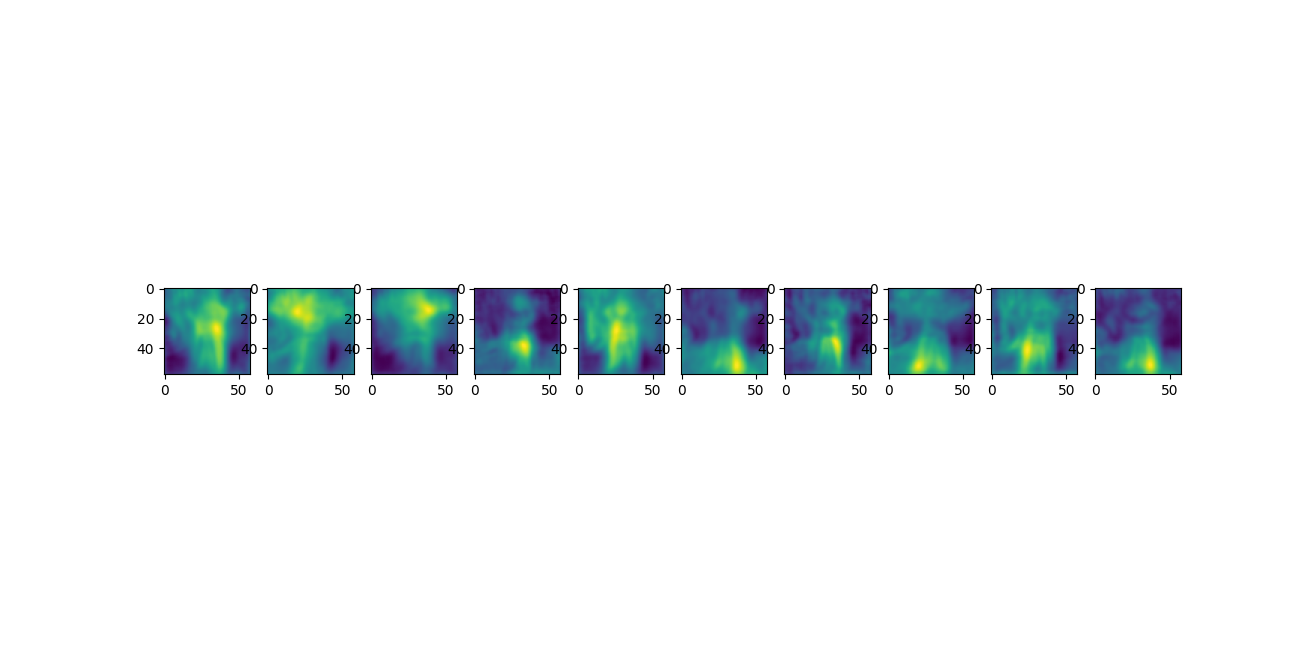
\includegraphics[width=\columnwidth]{visualizations/mask_10kp}}
\caption{
$K$ channels of the keypoint detector network used in
\cite{siarohin2020order}, before the softmax activation. Our main motion
prior in this project.
}
\label{mask-10kp}
\end{center}
\vskip -0.2in
\end{figure}

Summing over the channels, we get Figure~\ref{mask-sum}.

\begin{figure}[ht]
\vskip 0.2in
\begin{center}
\centerline{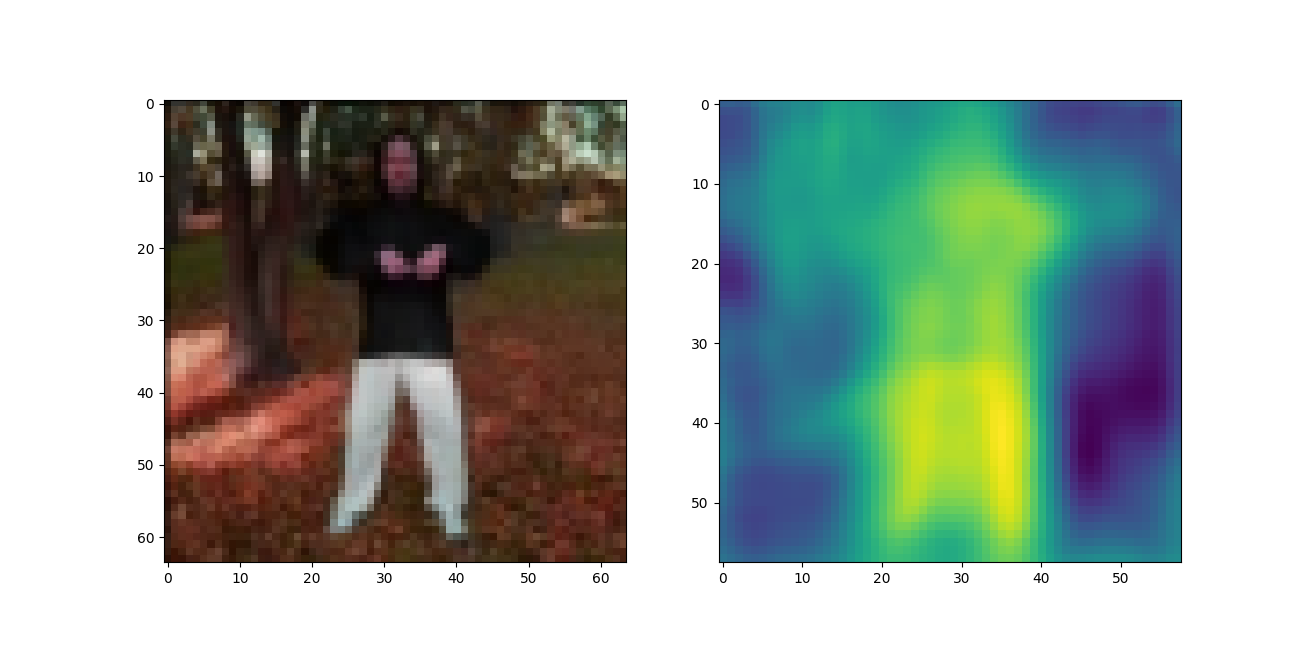
\includegraphics[width=\columnwidth]{visualizations/mask_sum}}
\caption{
The sum of the $K$ channels which is fed as a structural mask into the
generator.
}
\label{mask-sum}
\end{center}
\vskip -0.2in
\end{figure}
which is our output mask, aka the heatmap, pre softmax mask.

\subsection{Second mask version for relative motion transfer}
We purposes an additional "circles" only mask
which can be used in the context
of relative motion transfer during animation, as in
\cite{siarohin2020order}, which isn't possible with the previous heatmap mask.
The mask catches the geometry representation \cite{wu2019transgaga} of the
image, and by forcing it to be described as keypoints with a center, we can
use the relative coordinates for the animation. However, this module didn't
perform as well as our heatmap mask module (Table~\ref{table:results}).
Relative motion transfer isn't always the wanted outcome, but this work
indicates that a keypoint-only-prior based module is feasible for the task.
It can be expected that we will get results which are more similar to
\cite{siarohin2019animating}, due to the fact that the only information
that the pair of masks contain is the keypoint displacement, so our deep
network can only try its best to simulate a zero order approximation.

By taking the softmax over the heatmap, we get Table~\ref{softmax-10kp}.
\begin{figure}[ht]
\vskip 0.2in
\begin{center}
\centerline{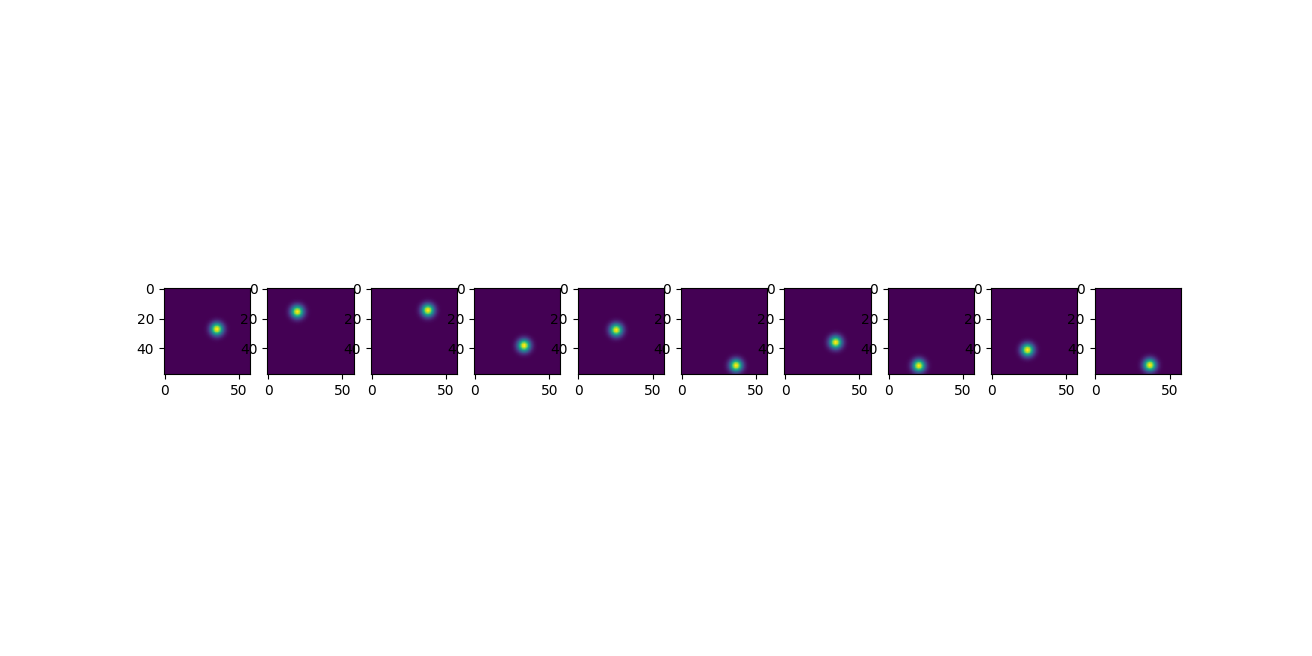
\includegraphics[width=\columnwidth]{visualizations/softmax_10kp}}
\caption{
$K$ channels of the keypoint detector network used in
\cite{siarohin2020order}, after the softmax activation and Gaussian fit.
}
\label{softmax-10kp}
\end{center}
\vskip -0.2in
\end{figure}

Summing over the channels, we get Table~\ref{softmax-sum}.

\begin{figure}[ht]
\vskip 0.2in
\begin{center}
\centerline{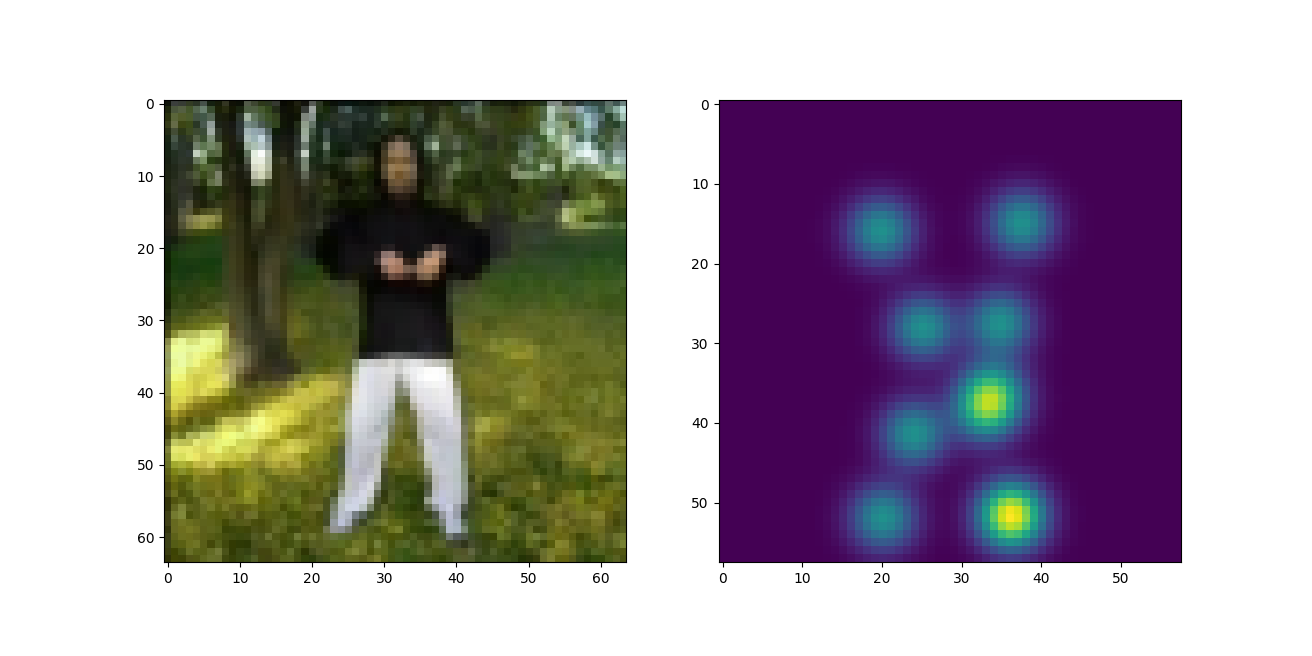
\includegraphics[width=\columnwidth]{visualizations/softmax_sumkp}}
\caption{
The sum of the $K$ channels which is fed as a structural mask into the
generator.
}
\label{softmax-sum}
\end{center}
\vskip -0.2in
\end{figure}
which is our output mask, aka the keypoints after softmax mask.

\subsection{Architecture}
\label{method}

\begin{figure}[ht]
\vskip 0.2in
\begin{center}
\centerline{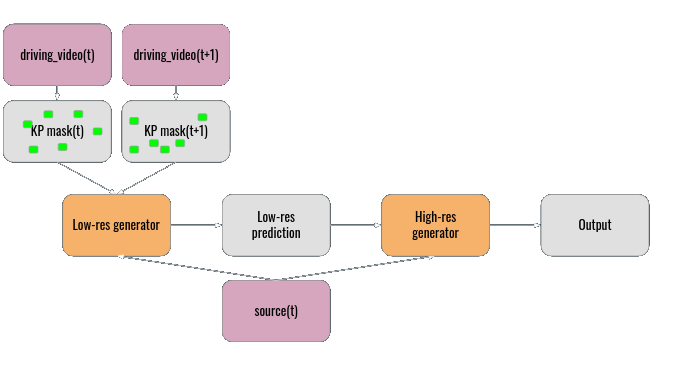
\includegraphics[width=\columnwidth]{visualizations/architecture}}
\caption{Architecture of the model. The keypoint mask can be either a
keypoint heatmap such as in Figure~\ref{mask-sum}, or drawn keypoint
circles as in Figure~\ref{softmax-sum}.}
\label{arch}
\end{center}
\vskip -0.2in
\end{figure}

Our architecture follows \cite{siarohin2020order} without the dense
motion module, after changing its keypoint generation module to return our
mask. After the mask is obtained, we follow the encoder decoder approach as
\cite{shalev2020image}.
Namely, the encoder of the low resolution generator consists of $\textit{conv}_{7
\times 7}$, $\textit{batch\_norm}$, $\textit{relu}$, followed by six
residual blocks of $\textit{batch\_norm}$, $\textit{relu}$,
$\textit{conv}_{3 \times 3}$ ,$\textit{batch\_norm}$, $\textit{relu}$,
$\textit{conv}_{3 \times 3}$, (and a sum with the source).
The residual blocks help to maintain the identity of the source image
\cite{he2015deep}.
The decoder consists of two blocks, each is a sequence of
$\textit{up\_sample}_{2 \times 2 }$, $\textit{batch\_norm}$,
$\textit{relu}$. The decoder is followed by a $\textit{conv}_{7 \times 7}$
and a $\textit{sigmoid}$ activation.
For the high resolution generator, use an encoder (decoder) with five encoding (decoding) blocks,
where each block is a sequence of
$\textit{conv}_{3 \times 3}$, $\textit{batch\_norm}$, $\textit{relu}$
$\textit{avg\_pool}_{2 \times 2}$, and each decoding block is a sequence of
$\textit{up\_sample}_{2 \times 2}$, $\textit{conv}_{3 \times 3}$,
$\textit{batch\_norm}$, $\textit{relu}$.
We add skip connections from each of the encoding layers to its
corresponding encoding layer, to form a U-Net architecture
\cite{ronneberger2015unet}.


\subsection{Losses}
We use the same perceptual loss as in \cite{siarohin2020order} which is
based on the implementation of \cite{wang2018videotovideo}. With the input
driving frame $D$ and the corresponding reconstructed frame $\hat{D}$, the
reconstruction loss is written as: $L_{rec}(\hat{D}, D) =
\sum_{i=1}^{I} |N_i(\hat{D})-N_i(D)|$, where $N_i(\cdot)$ is the $i^{th}$
channel feature extracted from a specific VGG-19 layer \cite{simonyan2015deep}
and $I$ is the number of feature channels in this layer. Additionally we use this lose on
a number of resolutions, forming a pyramid obtained by down-sampling
$\hat{D}$ and $D$, similarly to \cite{}, \cite{}. The resolutions are $256
\times 256$, $128 \times 128$, $64 \times 64$ and $32 \times 32$.


\section{Experiments}
\subsection{Datasets}
The training and evaluation were done using Tai-chi-HD dataset which
containing short videos of people performing Tai-chi exercises.
Following \cite{siarohin2020order}, 3,141 Tai-chi videos were downloaded from YouTube.
The videos were cropped and resized to a resolution of $256^2$, while preserving the aspect ratio. There are 3,016 training videos and 125 test videos.

\begin{table}[t]
\caption{Images comparison}
\label{table:images}
\vskip 0.15in
\begin{center}
\begin{small}
\begin{sc}
\begin{tabular}{m{1.0cm}m{1.0cm}m{1.0cm}m{1.0cm}m{1.0cm}m{1.0cm}}
\toprule
Source image & Driving\\
\toprule
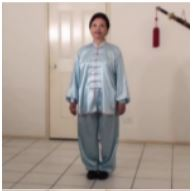
\includegraphics[width=1cm, height=1cm]{images/source} &
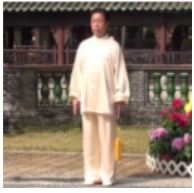
\includegraphics[width=1cm, height=1cm]{images/driving_1} &
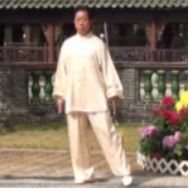
\includegraphics[width=1cm, height=1cm]{images/driving_2} &
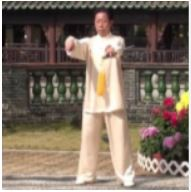
\includegraphics[width=1cm, height=1cm]{images/driving_3} &
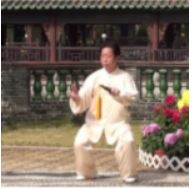
\includegraphics[width=1cm, height=1cm]{images/driving_4} &
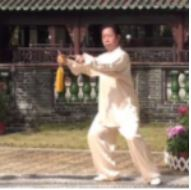
\includegraphics[width=1cm, height=1cm]{images/driving_5} \\
\midrule
X2Face & 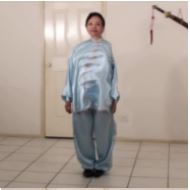
\includegraphics[width=1cm, height=1cm]{images/1_X2Face_1} &
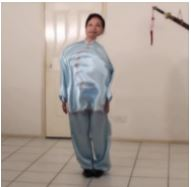
\includegraphics[width=1cm, height=1cm]{images/1_X2Face_2} &
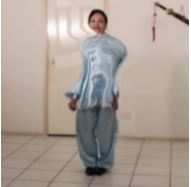
\includegraphics[width=1cm, height=1cm]{images/1_X2Face_3} &
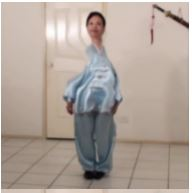
\includegraphics[width=1cm, height=1cm]{images/1_X2Face_4} &
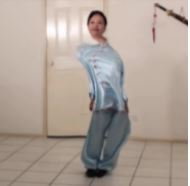
\includegraphics[width=1cm, height=1cm]{images/1_X2Face_5} \\
Monkey-Net & 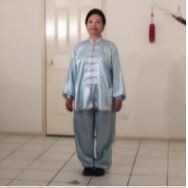
\includegraphics[width=1cm, height=1cm]{images/2_Monkey-Net_1} &
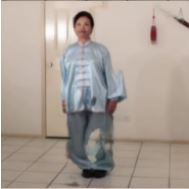
\includegraphics[width=1cm, height=1cm]{images/2_Monkey-Net_2} &
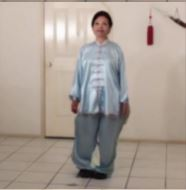
\includegraphics[width=1cm, height=1cm]{images/2_Monkey-Net_3} &
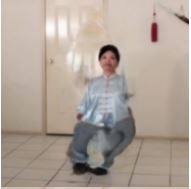
\includegraphics[width=1cm, height=1cm]{images/2_Monkey-Net_4} &
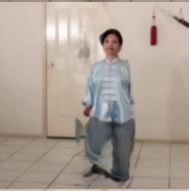
\includegraphics[width=1cm, height=1cm]{images/2_Monkey-Net_5} \\
FOMM & 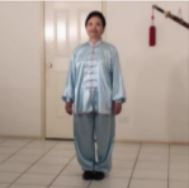
\includegraphics[width=1cm, height=1cm]{images/3_FOMM_1} &
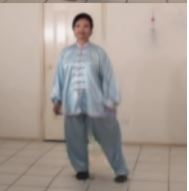
\includegraphics[width=1cm, height=1cm]{images/3_FOMM_2} &
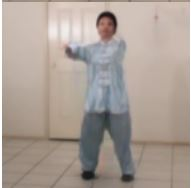
\includegraphics[width=1cm, height=1cm]{images/3_FOMM_3} &
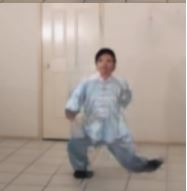
\includegraphics[width=1cm, height=1cm]{images/3_FOMM_4} &
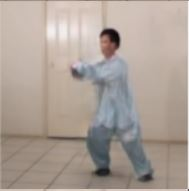
\includegraphics[width=1cm, height=1cm]{images/3_FOMM_5} \\
Perturbed Mask & 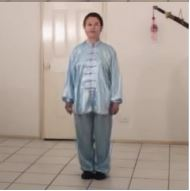
\includegraphics[width=1cm,
height=1cm]{images/4_Perturbed_1} &
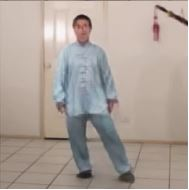
\includegraphics[width=1cm, height=1cm]{images/4_Perturbed_2} &
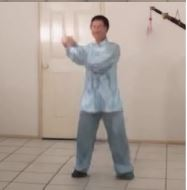
\includegraphics[width=1cm, height=1cm]{images/4_Perturbed_3} &
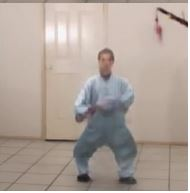
\includegraphics[width=1cm, height=1cm]{images/4_Perturbed_4} &
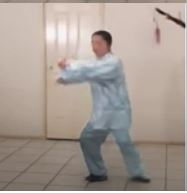
\includegraphics[width=1cm, height=1cm]{images/4_Perturbed_5} \\
Ours & 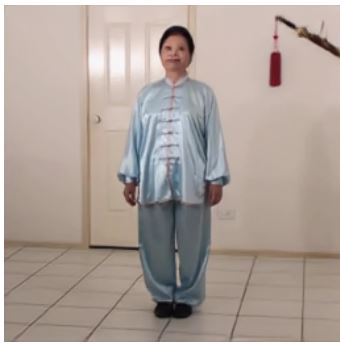
\includegraphics[width=1cm, height=1cm]{images/5_Ours_1} &
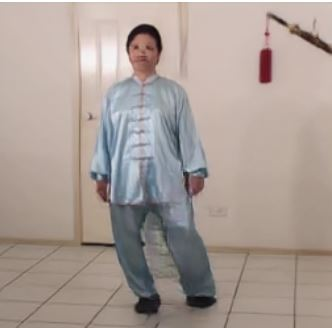
\includegraphics[width=1cm, height=1cm]{images/5_Ours_2} &
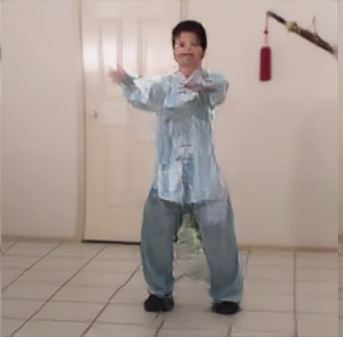
\includegraphics[width=1cm, height=1cm]{images/5_Ours_3} &
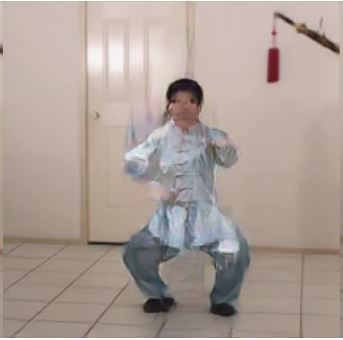
\includegraphics[width=1cm, height=1cm]{images/5_Ours_4} &
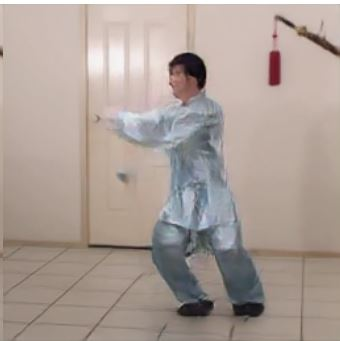
\includegraphics[width=1cm, height=1cm]{images/5_Ours_5} \\
\bottomrule
\end{tabular}
\end{sc}
\end{small}
\end{center}
\vskip -0.1in
\end{table}


\subsection{Comparison with Previous Works}
In order to compare our work to previous works (Table~\ref{table:results})
we used metrics previously used in similar papers.
Average Key-points Distance \cite{cao2017realtime} (AKD)
measures the average key-points distance between the generated video and
the source video. Average Euclidean Distance \cite{zheng2019joint} (AED)
measures the average euclidean distance
 between the representations of the ground-truth and generated videos in
 some embedding space. In addition, we added the L1 distance as well.
 Our AED and AKD metrics were calculated using the following repository:
 \url{https://github.com/AliaksandrSiarohin/pose-evaluation}
\\
Note that those metrics aren't optimal since one can easily improve
reconstruction by increasing the bottleneck, and we can see our
artifacts in animation results (Table~\ref{table:images}).
However, our pose did follow the driving video well, and to improve the
identity and background artifacts, we suggest some fixes in Section~\ref{future}.

% Note use of \abovespace and \belowspace to get reasonable spacing
% above and below tabular lines.

\begin{table}[t]
\caption{Accuracy Metrics}
\label{table:results}
\vskip 0.15in
\begin{center}
\begin{small}
\begin{sc}
\begin{tabular}{lcccr}
\toprule
Method & AKD & AED & L1 \\
\midrule
X2Face    & 17.654 & 0.272 & 0.080 \\
Monkey-Net    & 10.798 & 0.228 & 0.077 \\
FOMM    & 6.872 & 0.167 & 0.063 \\
Perturbed Mask & 4.239 & 0.147 & 0.047 \\
Ours (circles mask) & 14.760& 0.245 & 0.077 \\
Ours & 5.551 & 0.141 &  0.045\\
\midrule
Improvement (FOMM)    & 19.2\% & 15.5\% & 28.5\% \\
\bottomrule
\end{tabular}
\end{sc}
\end{small}
\end{center}
\vskip -0.1in
\end{table}
\section{Future work}
\label{future}
We would like to test our module on more datasets, and compare them to the
state of the art. In addition, summing the heatmap channels might not be
optimal, and there is certainly some space to try something deeper with the
features extracted in the keypoint detector as an input, or feed all of the
channels separately into the generator. We want to experiment with
mask thresholds due to the distortions in the animation background.
We may also increase the number of keypoints, but that would probably be
more beneficent to the second type of mask, and would increase the
required GPU memory proportionally. We also thought about coloring
matching keypoints with the same color to help the module to learn a motion
flow.

\section{Conclusions}
We constructed a novel method for image animation by moving the need for
a strong motion prior (optical flow) to the assumption of a pre-trained
keypoint detector/keypoint heatmaps prior to activation, which might be
based on a motion prior.
By doing so, we encapsulated motion to a motion mask, which is
bottlenecked by the prior training which has the keypoint bottleneck.
The motion masks are then fed into a generator, which combines the
appearance of the source image and the mask which represents the structure,
decoupled from any appearance naturally by the assumption that during the
training of the keypoint detector, the heatmap mask went into a keypoint
bottleneck. After evaluation, we can conclude that our method is
feasible, although with some artifacts.
\section*{Software and Data}
Detailed in our repository:
\\
\url{https://github.com/or-toledano/
animation-with-keypoint-mask}
\bibliography{animation-with-keypoint-mask}
\bibliographystyle{icml2021}

\end{document}
